\chapter{Vision Artificial}

\section{Camara}
Como se abordo al inicio de este proyecto, la cámara es la parte fundamental en
la captura de datos, suple la función de un ojo y depende de diversos
parámetros el que tengamos una captura de calidad. Para este trabajo profesional
la cámara que se utilizo fue la del fabricante HardKernel y que lleva de nombre
Ocam
\begin{center}
	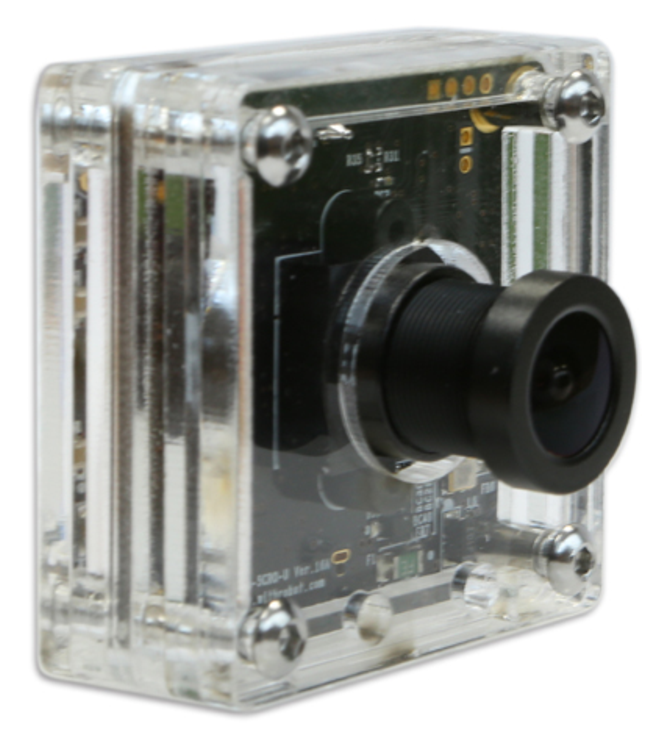
\includegraphics[width=0.3\textwidth]{Capitulo4/Fig0_1.eps}
	\captionof{figure}{Camara 'Ocam'}\label{Fig1}
\end{center}
Que tiene las siguientes especificaciones.
\begin{itemize}
	\item \textbf{Sensor:} CMOS image sensor.
	\item \textbf{Lente: } Lente estandar M12 distancia focal de 3.6mm.
	\item \textbf{Field of view: } 65 grados.
	\item \textbf{Tamaño del sensor: }0.25inch (3673.6 $\mu$m x 2738.4 $\mu$m)
	\item \textbf{Tamaño del pixel: } 1.4 $\mu$m x 1.4 $\mu$m.
	\item \textbf{Interfaz: }USB 3.0 Super-Speed.
	\item \textbf{Frame rate: }\\
	      1920 x 1080 a 30fps, 1280 x 720 a45fps, 640 x 480 a30fps
\end{itemize}
El acceso directo a la memoria a través de USB 3.0 permite que los datos se
escriban en la memoria principal sin pasar por la CPU. Reduce significativamente
la carga de trabajo de la CPU.

\section{Algoritmo general}
\begin{algorithm}
	\caption{Algoritmo general del sistema de vision}
	\begin{algorithmic}[1]
		\State{Calibrar camara}
		\State{Capturar frame a 60fps}
		\State{Publicar frame en ROS}
		\State{Suscribirse al nodo publicador}
		\State{Convertir RGB a HSV}
		\State{Acotar el modelo HSV al color de elección}
		\State{Agregar filtro morfologico}
		\State{Obtener centroide de la figura obtenida en 6}
		\State{Publicar coordenadas del centroide}
	\end{algorithmic}
\end{algorithm}

% ---------------------------------------------------------------------------------------------------------
% *********************************************************************************************************
% *********************************************************************************************************
% ---------------------------------------------------------------------------------------------------------

\section{Calibración de camara}


% ---------------------------------------------------------------------------------------------------------
% *********************************************************************************************************
% *********************************************************************************************************
% ---------------------------------------------------------------------------------------------------------


\section{Comunicación con ROS}
En la sección de vision artificial se lanzan dos nodos, uno encargado de capturar y
publicar frames a 60hz y el otro que se suscribe a dicho nodo y realiza un procesamiento
con la información obtenida para posterior publicar coordenadas.
\begin{center}
	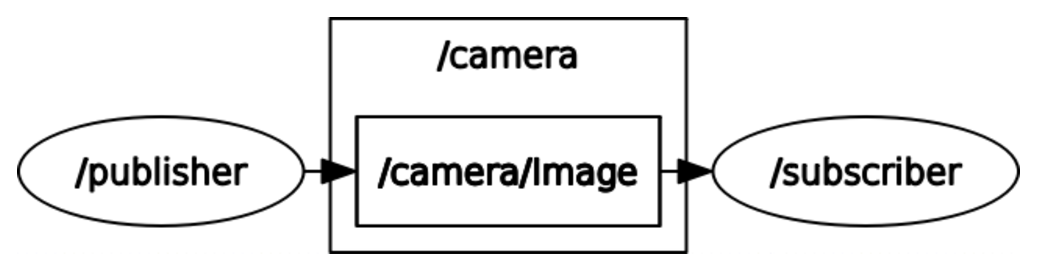
\includegraphics[width=0.6\textwidth]{Capitulo4/Fig0.eps}
	\captionof{figure}{Nodos y topic}\label{Fig1}
\end{center}
En la figura 4.1 se puede observar dos nodos conectados por un topic llamado /Image
encargado de comunicar la imagen de un nodo a otro.
\subsection{Publisher}
Como vimos anteriormente opencv es una libreria open-source que se encarga del procesamiento
de imagenes, también abordamos un poco acerca de como ROS comunica nodos y los
tipos de datos que puden ser publicados. Al hablar de que se va a publicar una imagen
estamos refiriendonos a una matriz que en este caso sera de 640 x 480.\\
ROS pasa las imágenes en su propio formato sensor\_msgs/Image , pero
en este caso usaremos ROS junto con las librerias de  OpenCV. CvBridge es una
biblioteca ROS que proporciona una interfaz entre ROS y OpenCV.
\begin{center}
	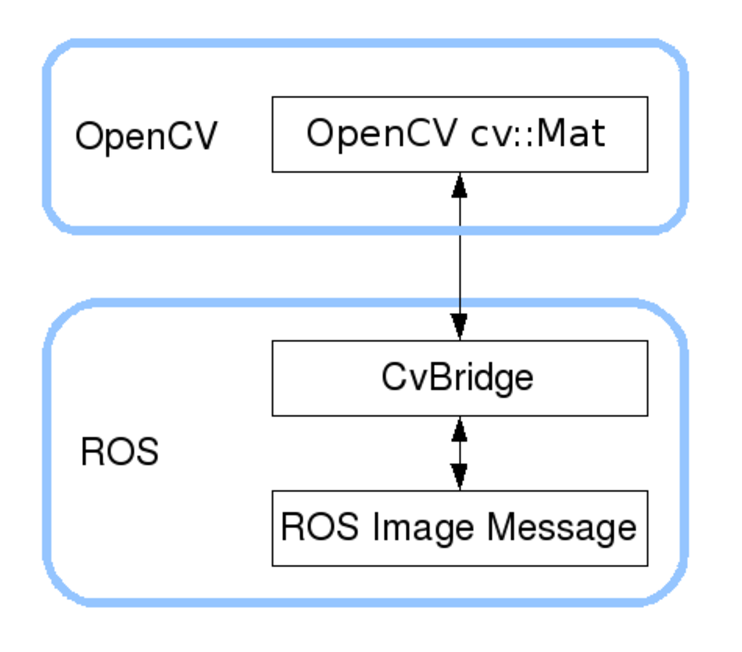
\includegraphics[width=0.5\textwidth]{Capitulo4/Fig1.eps}
	\captionof{figure}{Comunicación entre opencv y ROS}\label{Fig1}
\end{center}
Al convertir un mensaje sensor\_msgs/Image en una imagen Cv, CvBridge
reconoce dos casos de uso distintos:
\begin{itemize}
	\item Queremos modificar los datos en el lugar.\\
	      \textbf{Tenemos que hacer una copia de los datos del mensaje ROS.}
	\item No modificaremos los datos.\\
	      \textbf{Podemos compartir con seguridad los datos que posee el mensaje ROS en lugar de copiarlos.}
\end{itemize}

La entrada es el puntero del mensaje de imagen, así como un argumento de
codificación opcional. La codificación se refiere al destino CvImage.\\
Para codificaciones de imágenes populares, CvBridge opcionalmente realizará
conversiones de color o profundidad de píxeles según sea necesario. Para este proyecto
se utiliza bgr8: CV\_8UC3, es decir, que el orden del color es Azul, Verde y Rojo.\\
Con el fin de entender este nodo se hizo el siguiente diagrama de flujo:
\begin{center}
	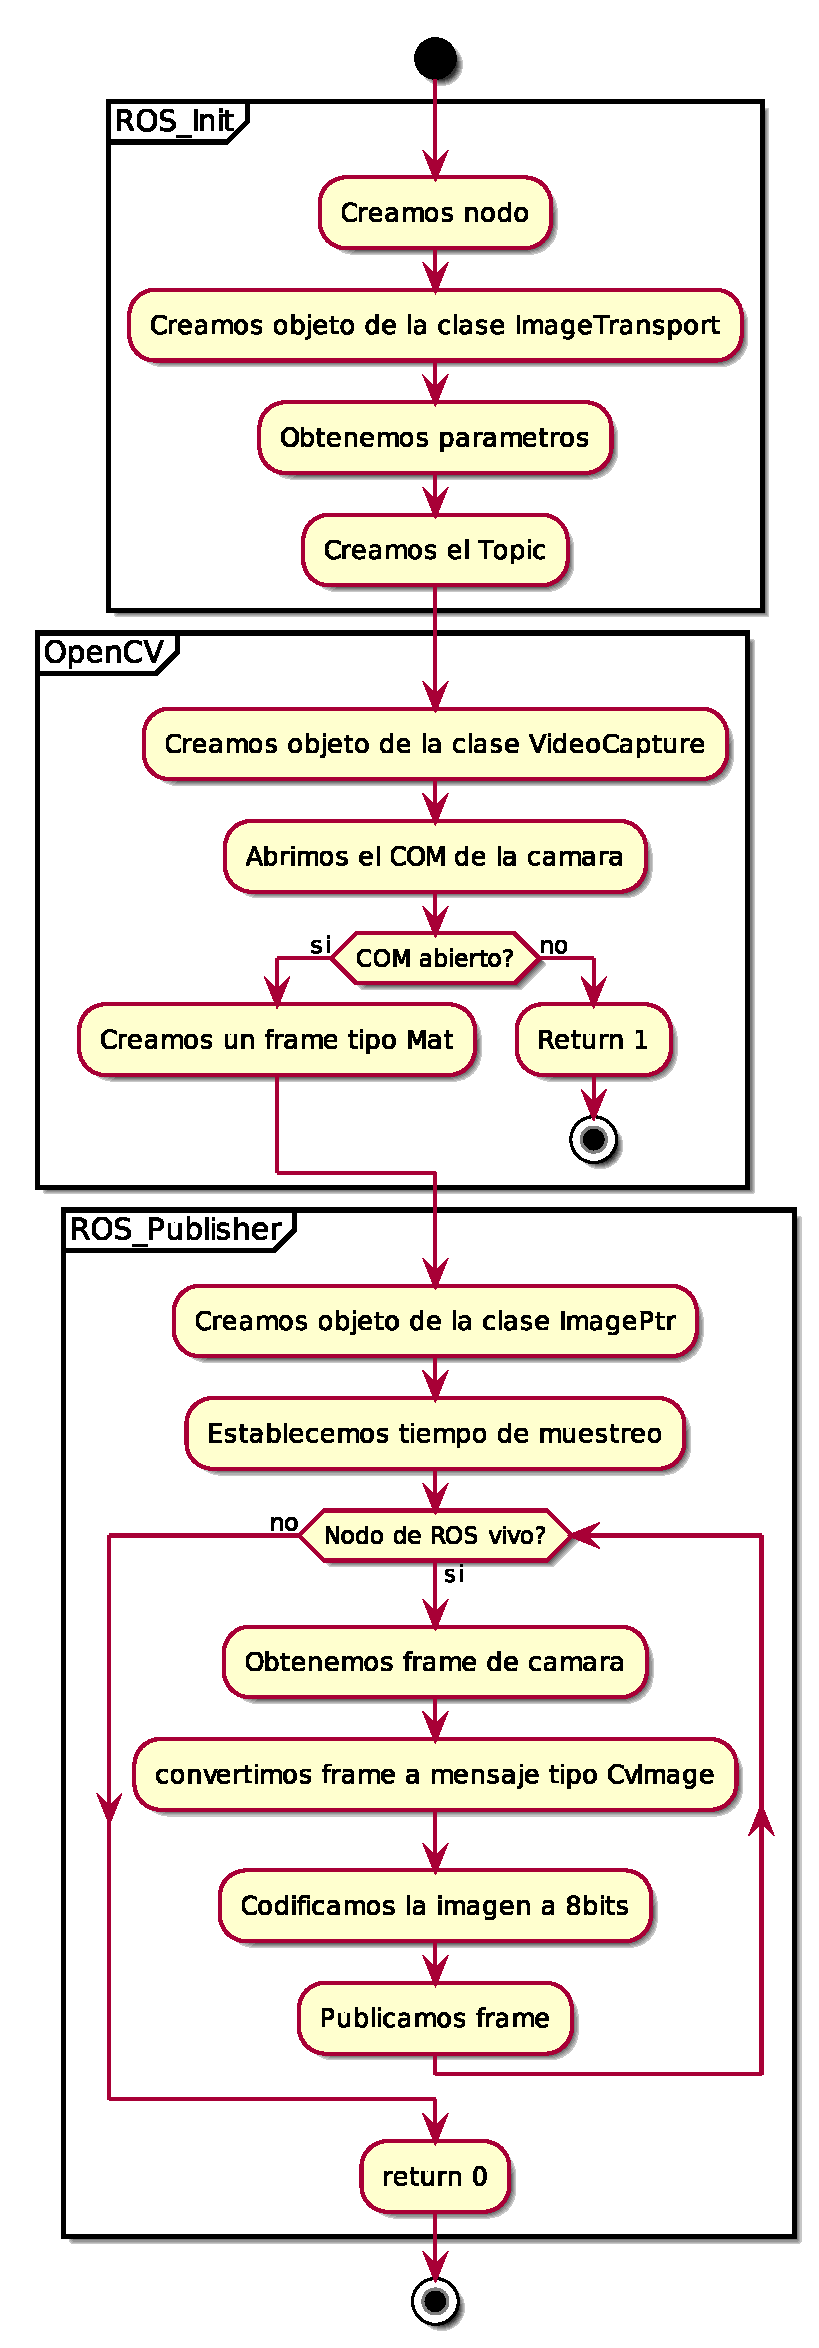
\includegraphics[width=0.35\textwidth]{Capitulo4/publisher.eps}
	\captionof{figure}{Diagrama de flujo del programa publisher}\label{Fig5}
\end{center}
El codigo se encuentra en la parte del Apendice A, 'codigo1'

\subsection{Subscriber}
Este nodo tiene dos funciones principales, Suscribirse al nodo publisher y publicar
un array de tamaño 2 tipo entero que guardara las coordenadas en X y Y del centroide
del target.\\
El proceso que se ejecuta se vera más a detalle en las siguientes secciones de este
capitulo.

% ---------------------------------------------------------------------------------------------------------
% *********************************************************************************************************
% *********************************************************************************************************
% ---------------------------------------------------------------------------------------------------------

\section{Espacio de color}
Como se puede apreciar en el algoritmo general, el paso 5 es el cambio de espacio de color
de RGB a HSV, además ya sabemos el porque es mejor generar colores partiendo del
modelo HSV. Así que lo que ahora sigue es la implementación en código y las pruebas
que se hicieron para tener un rango de colores y así tener una base de datos a la
cual recurriremos después.\\
El siguiente digrama muestra el flujo que el programa 2(ver apendice A) siguio para
el cambio de espacio de color.
\begin{center}
	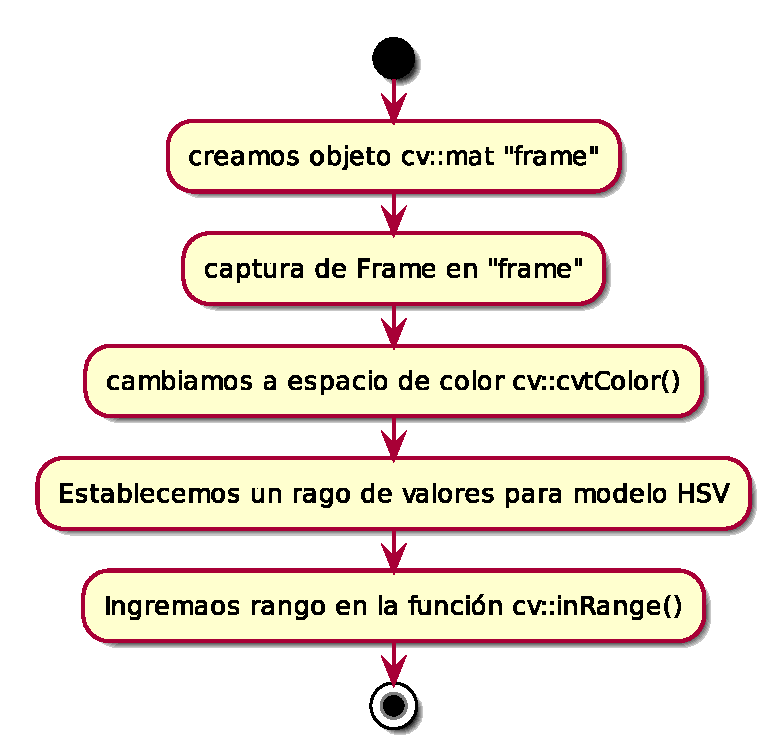
\includegraphics[width=0.5\textwidth]{Capitulo4/color.eps}
	\captionof{figure}{Diagrama de flujo para cambio de espacio de color}\label{color}
\end{center}
Empezamos con la función definida que nos dan las libreias de opencv para transformar
de RGB a HSV.
\begin{center}
	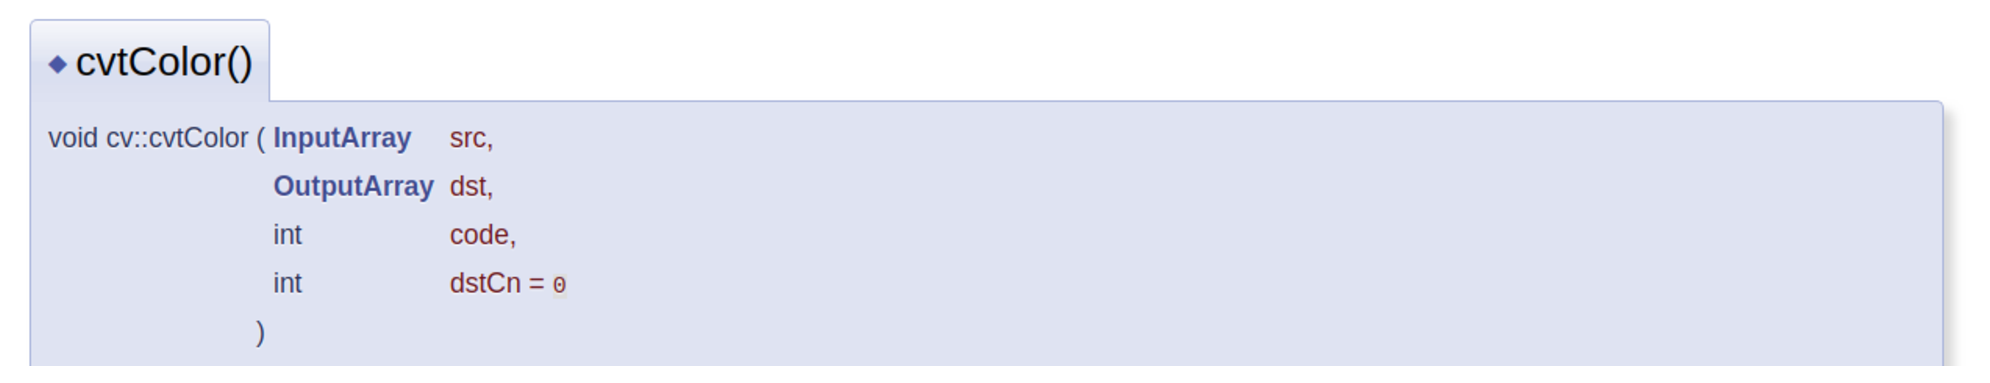
\includegraphics[width=0.85\textwidth]{Capitulo4/Fig2.eps}
	\captionof{figure}{Función Color \cite{opencvcolor}}\label{Fig2}
\end{center}
Donde
\begin{itemize}
	\item \textbf{src}: Imagen de entrada de 8 bits sin signo
	\item \textbf{sdt}: Imagen de salida del mismo tamaño y profundidad que src.
	\item \textbf{code}: Código de conversión de espacio de color en este caso es \\COLOR\_BGR2HSV.
	\item \textbf{dstCn}: Número de canales en la imagen de destino; si el parámetro es 0, el
	      número de canales se deriva automáticamente de src y código.
\end{itemize}

El formato de color predeterminado en OpenCV a menudo se denomina RGB, pero en realidad
es BGR (los bytes se invierten). Entonces, el primer byte en una imagen en color estándar
(24 bits) será un componente azul de 8 bits, el segundo byte será verde y el tercer
byte será rojo. El cuarto, quinto y sexto bytes serían el segundo píxel (Azul, luego
Verde, luego Rojo), y así sucesivamente.\\
Ahora pasamos a la función que acota el color que deseemos, esta es la llamada inRange()
\begin{center}
	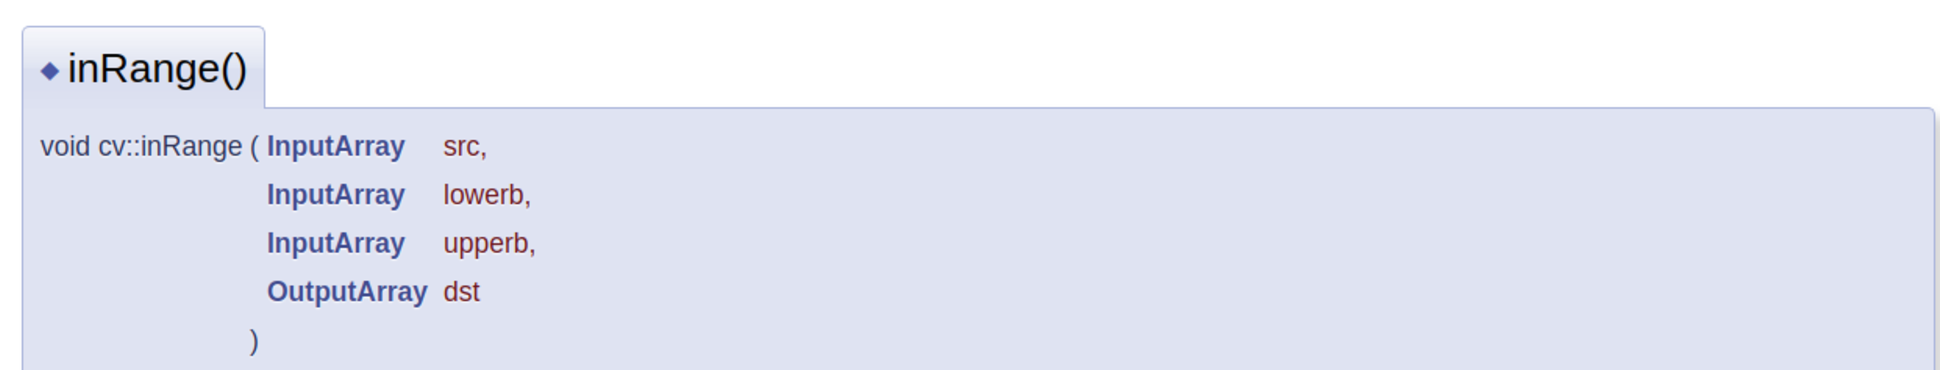
\includegraphics[width=0.9\textwidth]{Capitulo4/Fig3.eps}
	\captionof{figure}{Función inRange}\label{Fig6}
\end{center}
Donde
\begin{itemize}
	\item \textbf{src} primera matriz de entrada.
	\item \textbf{lowerb} matriz de límite inferior o un escalar.
	\item \textbf{upper}  matriz de límite superior o un escalar.
	\item \textbf{dst} Conjunto de salida dst del mismo tamaño que src y tipo CV\_8U.
\end{itemize}
Debido a que no hay un solo color azul o rojo, etc, si no más bien un rango que cubre
la gama de azules, amarillo, naranja, etc. Por esa razón se hicieron pruebas para
determinar los valores HSV que corresponden a los siguientes colores: Amarillo, Azul,
Rojo, Verde y Naranja y de esta manera a la hora de seguir un objetivo de dado color
el sistema no tenga problemas en reconocer esa gama de color.\\
La siguiente figura ilustra una gama de colores que va desde el rojo al azul, donde la
tarea es obtener un conjunto de imagenes que correspondan a un sector de la misma.
\begin{center}
	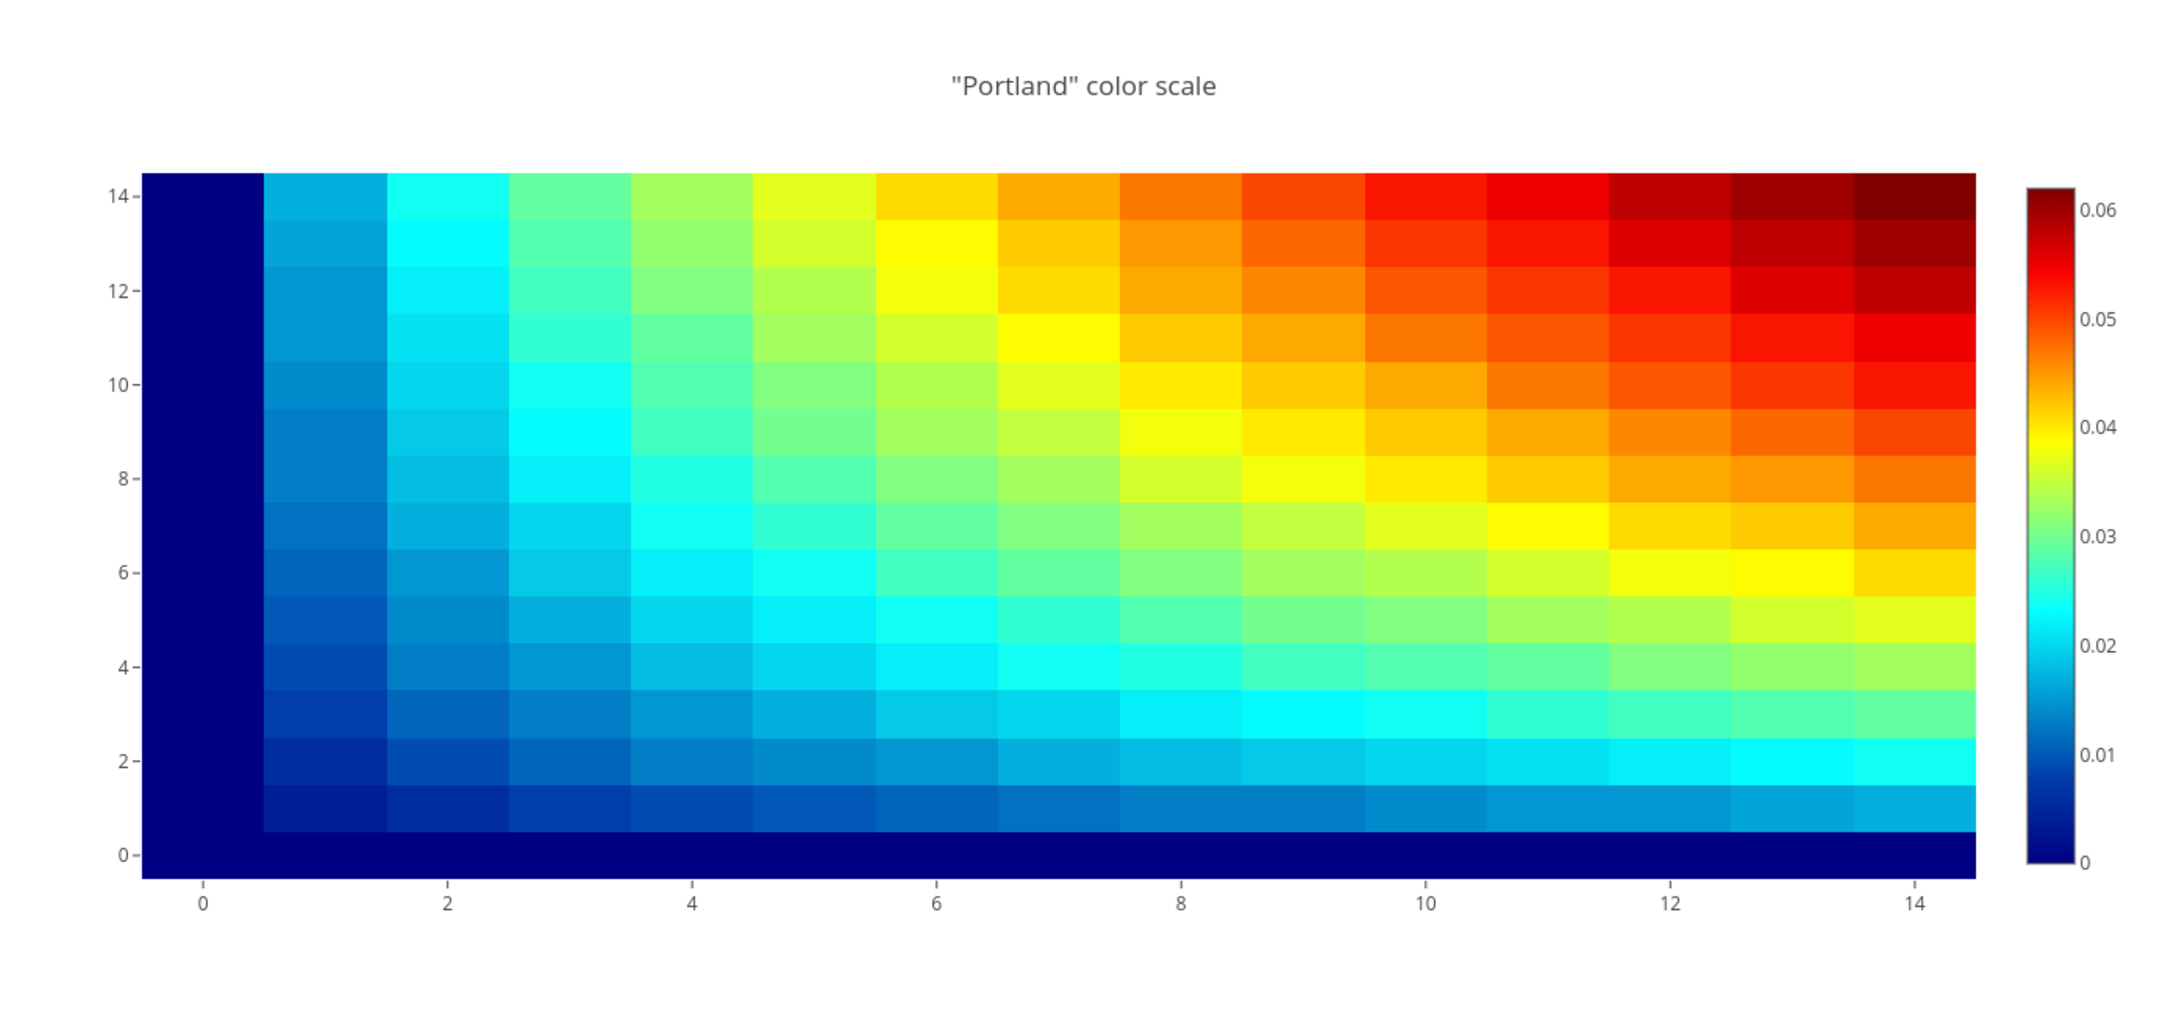
\includegraphics[width=0.6\textwidth]{Capitulo4/Fig4.eps}
	\captionof{figure}{Espectro de colores}\label{Fig6}
\end{center}
De donde apartir del código 2 se obtuvieron los siguientes resultados.
\begin{center}
	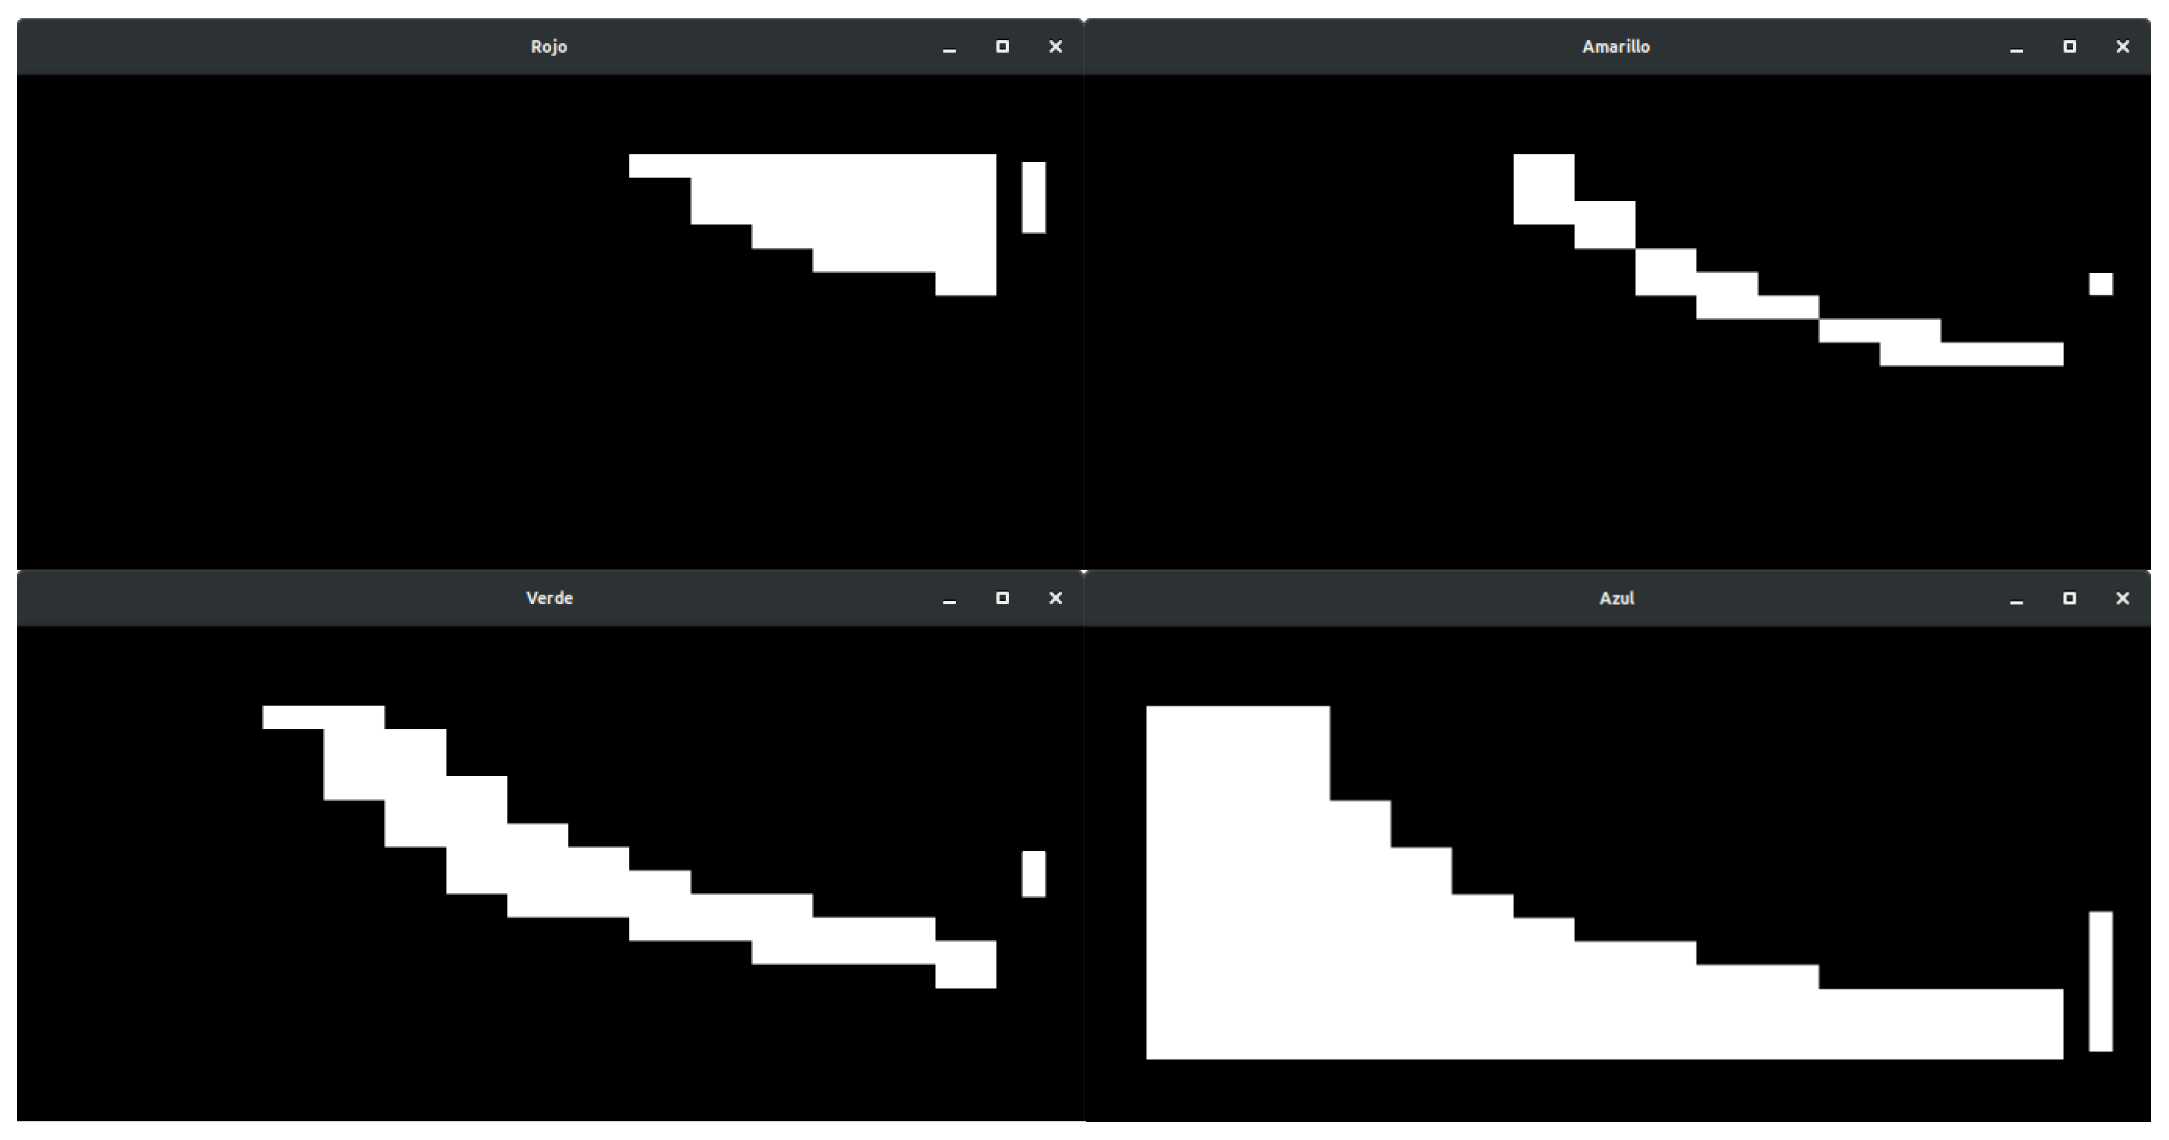
\includegraphics[width=0.6\textwidth]{Capitulo4/Fig5.eps}
	\captionof{figure}{Separación de colores}\label{Fig6}
\end{center}
En la figura 4.9 se aprecia la separación en 4 colores; Rojo, Amarillo, Verde y Azul.
con los siguientes rangos de valores.\\
\begin{table}[ht]
    \begin{center}
        \caption{A table without vertical lines.}
        \begin{tabular}[t]{lcccccc}
        \hline
        &H$_{min}$ & H$_{max}$ & S$_{min}$ & S$_{max}$ & V$_{min}$ & V$_{max}$ \\
        \hline
        Rojo & 0 & 10 & 100 & 255 & 100 & 255 \\
        Amarillo & 25 & 35 & 50 & 255 & 50 & 255 \\
        Verde & 35 & 75 & 100 & 255 & 100 & 255 \\
        Azul & 75 & 130 & 55 & 255 & 55 & 255 \\
        \hline
        \end{tabular}  
    \end{center}
\end{table}\\
A manera de tener una mejor visualización de los resultados, la siguiente figura concatena
cada segmento de color y le asigna un color plano a cada uno.
\begin{center}
	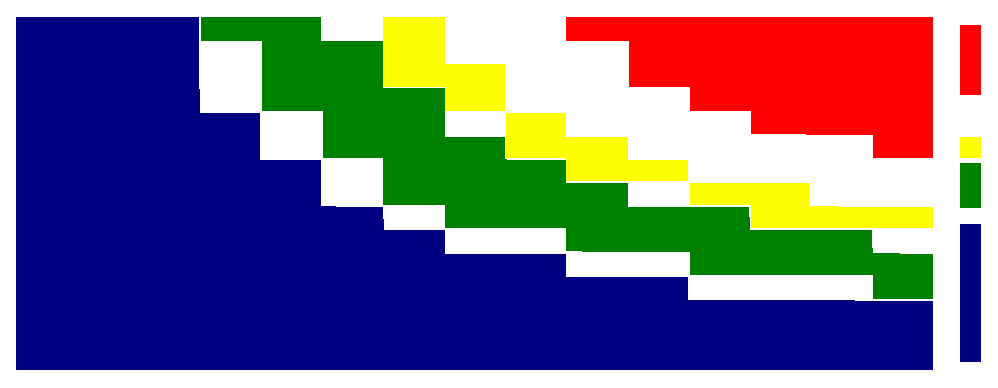
\includegraphics[width=0.6\textwidth]{Capitulo4/Fig6.eps}
	\captionof{figure}{Separación de colores}\label{Fig6}
\end{center}
